Logiikka laskee halutun juoman massan kaavalla
\begin{align}
    \mathrm{pourWeight} = \mathrm{pourAmount} \cdot 10 - 27 \mathrm{,}
\end{align}
eli halutusta massasta vähennetään vaa'an hitautta kuvaava vakio 27. Hitaus johtuu muun muassa tietoliikenneyhteyden hitaudesta ja silmukoiden sisällä olevista odotusajoista. Esimerkiksi robotin jobissa olevan timer-komennon tai logiikassa olevan sleep-komennon arvoa nostamalla tuo vakio 27 kasvaisi. Tämä hitaus tarkoittaa sitä, että pullon suoristusliikkeen aikana tapahtuviin muuttujiin ei pystytä enää vaa'an avulla vaikuttamaan. Käytännössä siis 27 grammaa juomaa kaatuu vielä sen jälkeen, kun logiikka havaitsee juomaa olevan tarpeeksi. Tämä on kuitenkin vain pieni osa koko kaatoliikettä. Esimerkiksi kaatonokan vaihtaminen sellaiseen kaatonokkaan, jossa virtausnopeus on eri, aiheuttaa sen, että tuo vakio muuttuu hieman.

Painoanturin tarkkuutta testattiin vertailemalla vaa'an antamia tuloksia tavallisen keittiövaa'an näyttämän painon kanssa. Kaikissa tapauksissa painoanturin ja keittiövaa'an tulos erosi maksimissaan yhdellä grammalla toisistaan. Vaa'an osoittamiin lukemiin saattaa tulla pieni impulssin aiheuttama piikki kaadon alussa, kun juomavirta ensimmäisenä osuu lasiin.

HandlePour-funktio taaraa vaa'an ennen jokaista kaatoa. Tämän ansiosta useamman komponentin juomasekoituksia on mahdollista kaataa tällä systeemillä. Funktiossa oleva currentWeight on siis mukiin tullut paino sen jälkeen, kun kyseisen komponentin kaato on aloitettu. Taaraus mahdollistaa myös mukitelineen pitämisen vaa'an päällä ilman että sen massaa erikseen vähennetään saadusta painosta. Mukiteline auttaa siihen, ettei muki liikahda juomavirran vaikutuksesta. Samoin voitaisiin myös käyttää erilaisia, eri painoisia mukeja ilman että se vaikuttaa kaatoihin. Kuvassa \ref{fig:kaato} näkyy robotti kaatamassa vaa'an päällä olevaan mukiin, joka on mukitelineessä.

\newpage

\begin{figure}[h]
\begin{center}
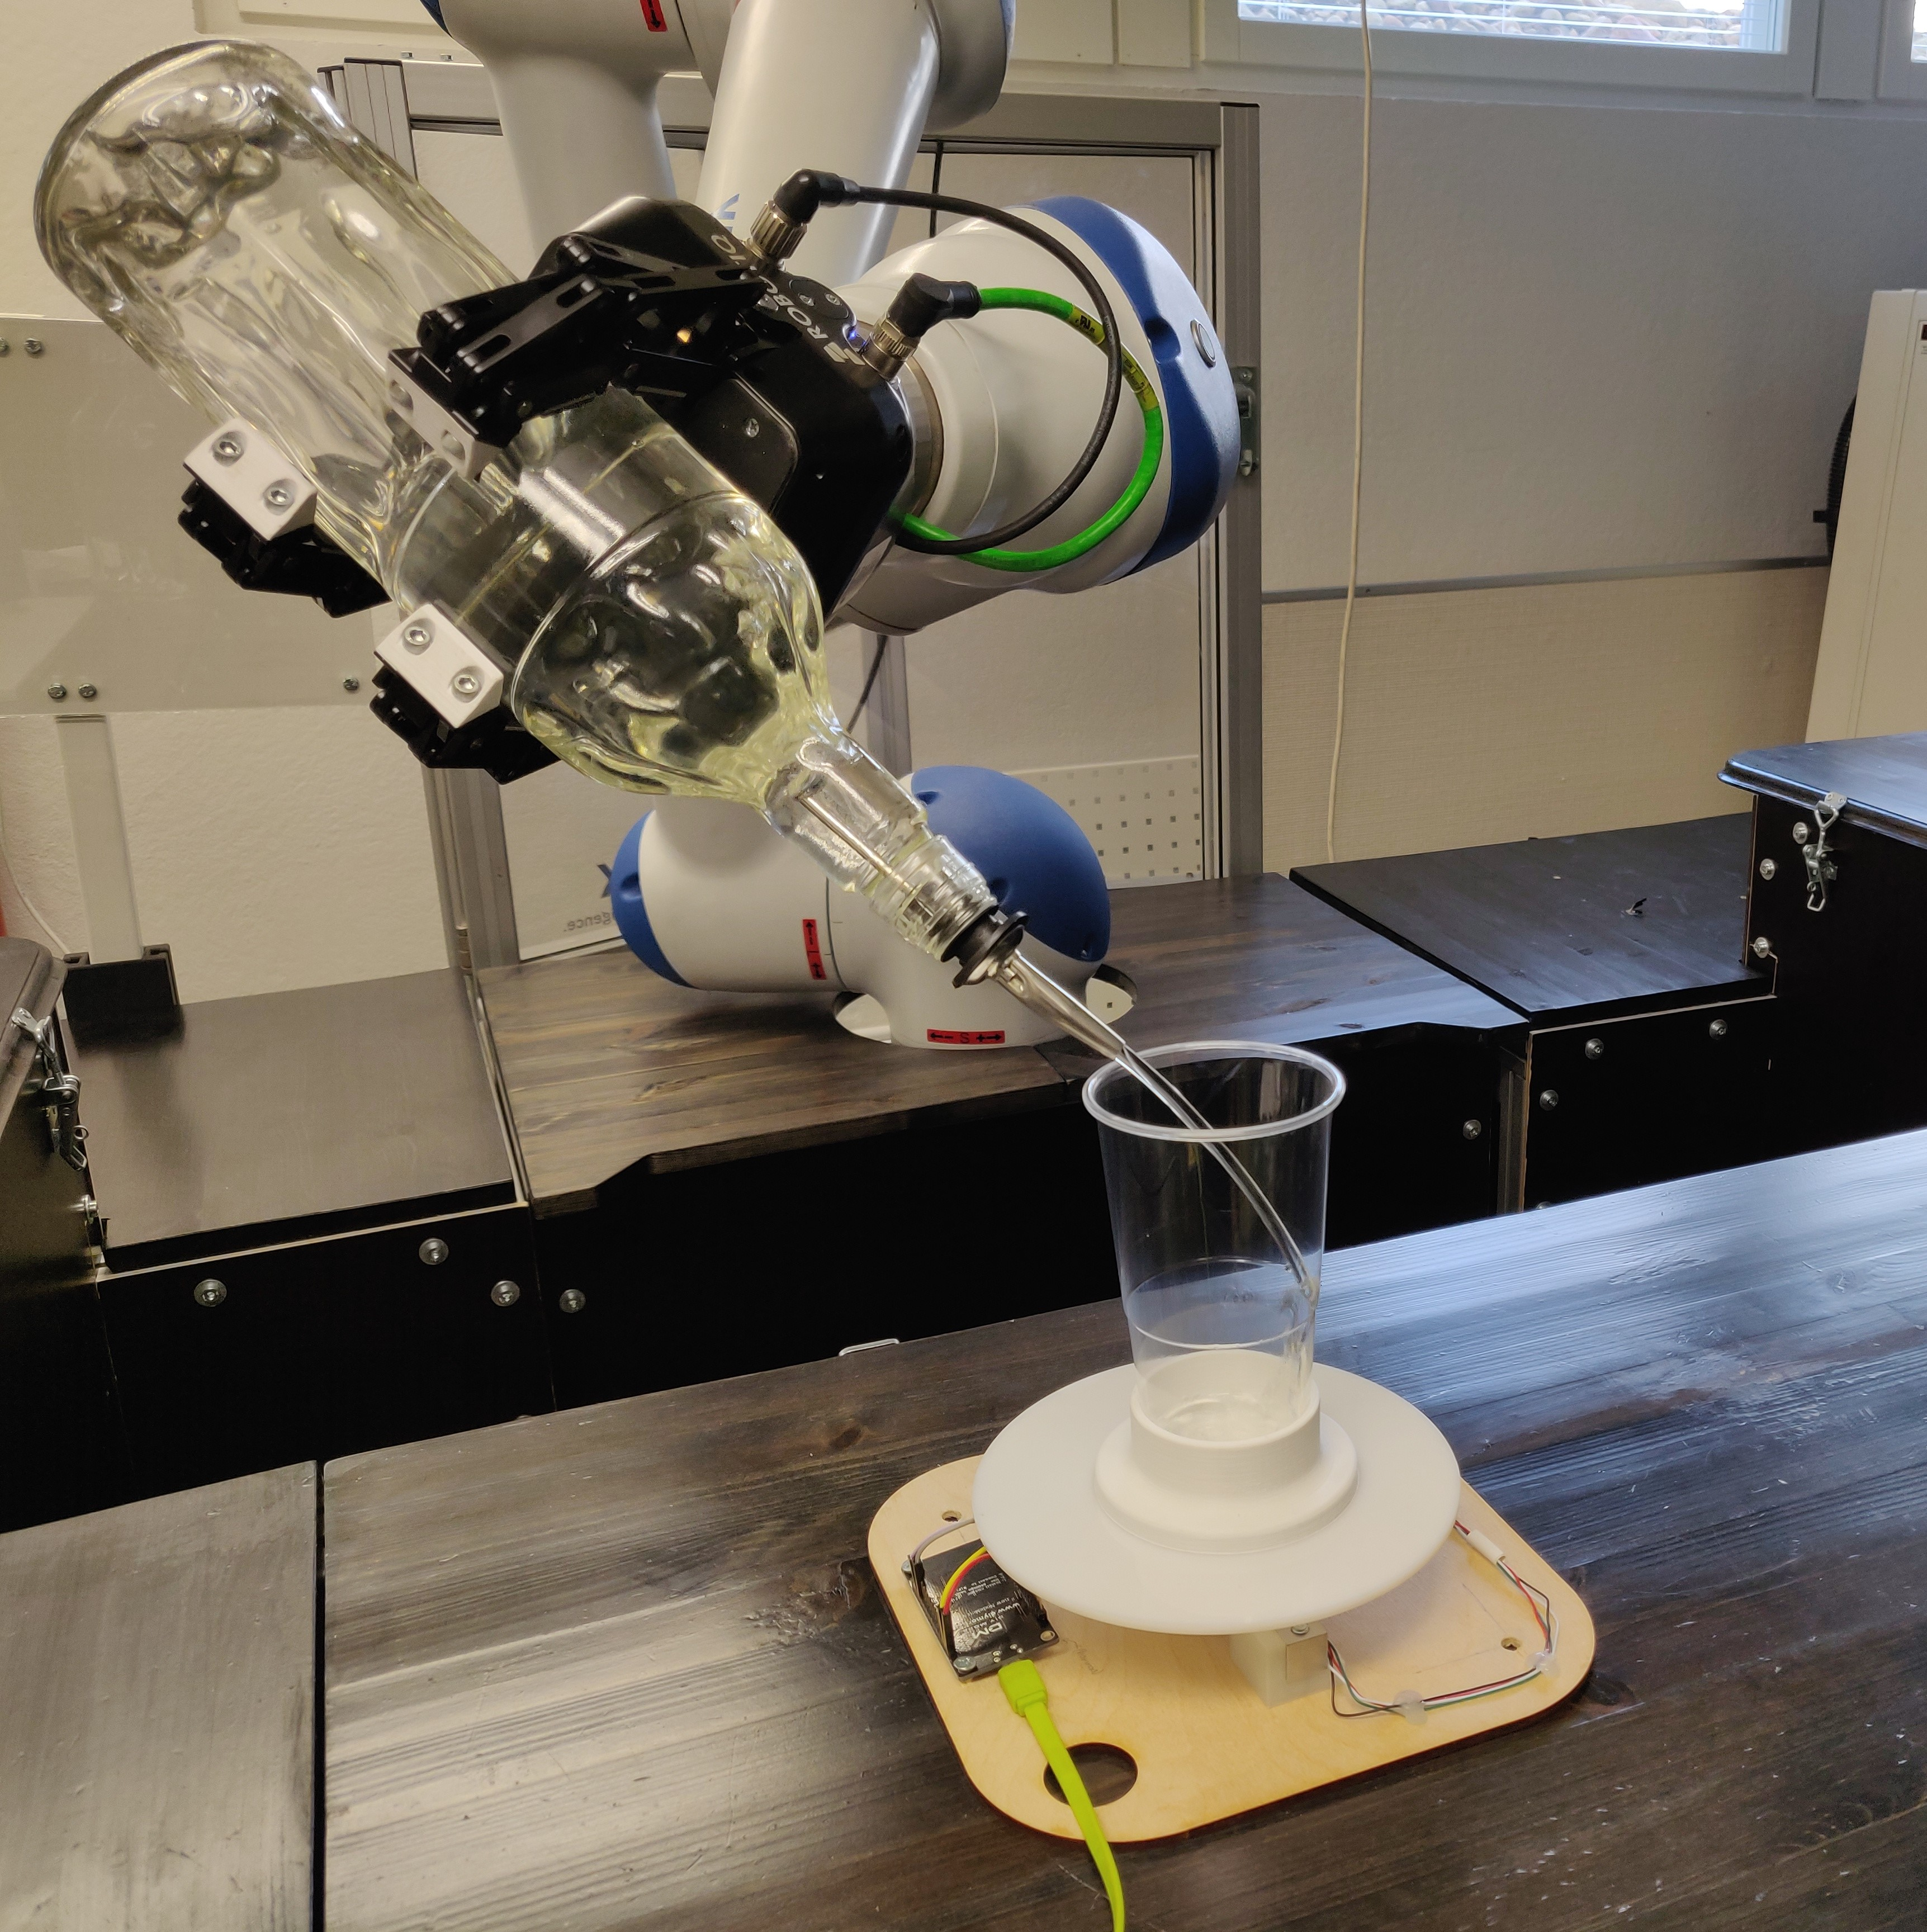
\includegraphics[scale=0.1]{img/kaato.jpg}
\end{center}
\caption{Robotti kaatoasennossa kaatamassa vaa'an päällä olevaan mukiin}
\label{fig:kaato}
\end{figure}

Uusi kaatosysteemi ei tällaisenaan mahdollista alle kolmen senttilitran kaatoja robotilla. Tämä johtuu siitä, että pelkkä kallistus- ja suoristusliikkeen aikana pullosta virtaava juoma on tilavuudeltaan noin kolme senttilitraa, vaikka robotti ei pysyisi kaatoasennossa paikallaan. Pienempiä kaatoja olisi luultavasti mahdollista saada muokkaamalla kaatoasennon kulmaa pienemmäksi. Kappaleessa \ref{ch:vanhan_ongelmat} luetellut lakisääteiset alkoholijuomien perusannokset eivät kuitenkaan vaadi alle neljän senttilitran kaatoja. Tämän takia pienten kaatojen mahdollisuutta ei lopulta ole tässäkään työssä toteutettu.
